The simulator in TVB resembles popular neural network simulators in 
many fundamental ways, both mathematically and in terms of informatics 
structures, however we have found it necessary to introduce auxiliary
concepts particularly useful in the modeling of large scale brain 
networks. In the following, we will highlight some of the interesting
principles and capabilities of TVB's simulator and give rough characterization
of the execution time and memory required in typical simulations.

\subsection{Node dynamics}

	In TVB, nodes are not considered to be abstract neurons nor necessarily
	small groups thereof, but rather large populations of neurons. Concretely,
	the main assumption of the neural mass modeling approach in TVB is that
	large pools of neurons on the millimeter scale are strongly approximated
	by population level equations describing the major statistical modes of
	neural dynamics \cite{Freeman_1975book}. Often, averaging techniques are
	employed, though techniques retaining several modes have been developed
	\cite{Stefanescu_2008, Stefanescu_2011}. Such an approach is certainly not
	new; one of the early examples of this approach consist of the well known
	Wilson-Cowan equations \cite{Wilson_1973}. Nevertheless, there are
	important differences in the the assumptions and goals from modeling of
	individual neurons, where the goal may be to reproduce correct spike
	timing or predict the effect of  a specific neurotransmitter. A second
	difference lies in coupling: chemical coupling is often assumed to be
	pulsatile, or discrete, between neurons, whereas it is considered
	continuous. Typically the goal of neural mass modeling is to study the
	dynamics that emerge from the interaction of two or more neural masses and
	the network conditions required for stability of a particular
	spatiotemporal pattern. In the following, we shall  briefly discuss some
	of the models available in TVB.

	As we have noted, many neural mass models have been developed. One of
	the more prominent examples in the systems neuroscience literature is 
	that the Jansen-Rit model of rhythms and evoked responses arising from
	coupled cortical column \cite{Zetterberg_1978, Jansen_1995, Spiegler_2010}. 
	\note[mw]{Continue description}.
	\note[psl]{maybe see David et al, 2004 for better description of local connectivity in the Jansen and Rit model}
	Advantages of the Jansen-Rit model stem from the connection made
	between empirical studies of neural tissue and the model's parameters, 
	making it easier in certain cases to make concrete predictions about
	the relation between a dynamical regime and its neurobiological 
	mechanism. However, because the form of the model used often employs
	at least six dimensions, it is not always clear how to analyze or
	visualize. Lastly, the model requires frequent computation of exponentials,
	requiring considerable computational time. 

	For these reasons, it is often desirable to have a simpler mathematical 
	model, which may be reproduce the same qualitative phenomena as other 
	models, implemented with fewer and simpler equations. Such is the motivation
	for the generic two-dimensional oscillator model provided by TVB. 
	Model produces oscillations, damped, spike-like or 
	sinusoidal activations. While these alone are not interesting, they 
	permit the study of network phenomena, such as synchronization of rhythms
	or propagation of evoked potentials, while requiring less time to simulate.

	However, the modeler's goals may not lead to either the Jansen-Rit
	\cite{Jansen_1995, David_2003, David_2004} or generic 2D oscillator
	\cite{FitzHugh_1961, Nagumo_1962}, and several other mass models are
	provided by TVB: the previously mentioned Wilson-Cowan description of
	functional dynamics of neural tissue \cite{Wilson_1972}, the Kuramoto
	model describing synchronization \cite{Kuramoto_1975, Cabral_2011}, two
	and three dimensional mode-level models describing populations with
	excitability distributions \cite{Stefanescu_2011, Stefanescu_2008}, a
	reduction of the Wong and Wang model \cite{Wong_2006} as presented in
	\cite{Deco_2013} and a lumped version of Liley's model \cite{Liley_1999,
	Steyn-Ross_1999} model are among the available models in TVB.

	Again, should any of these be insufficient, a new model can be implemented
	with minimal effort by subclassing a base \texttt{Model} class and
	providing a  \texttt{dfun} method to compute the right hand sides of the
	differential  equations. Please refer to the \url{https://github.com/the-
	virtual-brain/scientific_library/tree/trunk/contrib/simulator/models} for
	examples. There, models found in the work of 
	\cite{Larter_1999, Breakspear_2003, Morris_1981, Hindmarsh_1984, Brunel_2001}
	have been implemented.

\subsection{Network structure}

	The network of neural masses in TVB simulations directly follows from  a
	pair of geometrical constraints on cortical dynamics. The first is the
	large-scale white matter fibers that form a non-local and heterogeneous
	(translation variant) connectivity, either measured by anatomical tracing
	(CoCoMac\ref{CoCoMac}) or diffusion-weighted imaging \cite{Hagmann_2008,
	Honey_2009, Bastiani_2012}. The second is that of horizontal projections
	along the surface, which are modeled through a translation invariant
	\note[sk]{Not technically true, using singular parameters will produce
	this but that's only a limited subset of the capability, spatially
	inhomogeneous parameters are supported -- thus being more general than the
	restricted case of translational invariance} connectivity kernel,
	approximating a neural field.

	\subsubsection{Large-scale connectivity}

	The large-scale region level connectivity at the scale of centimeters,
	resembles more a traditional neural network than a neural field in that
	neural space is discrete,  each node corresponding to a neuroanatomical
	region of interest, such as V1, etc. It is at this level that inter-regional 
	time delays play a large role, whereas the time delays due to 
	lateral, local projections are subsumed under the dynamics of the node.

	It is often seen in the literature that the inter-node coupling functions
	\textit{are} part of the node model itself. In TVB, we have instead 
	chosen to factor such models into the intrinsic neural mass dynamics, where each 
	neural mass's equations specify how connectivity contributes to the
	node dynamics, and the coupling function, which specifies how the activity
	from each region is mapped through the connectivity matrix. Common coupling 
	functions are provided such as the linear, difference and periodic functions
	often used in the literature.

	\subsubsection{Local connectivity}

	The local connectivity of the cortex at the scale of millimeters provides
	a continuous 2D surface along horizontal projections connect 
	cortical columns. Such a structure has previously been modeled by
	neural fields \cite{Amari_1977, Jirsa_1997, Liley_1999}. In TVB, a cortical mesh, 
	as obtained from structural MRI data and simplified, provides a spatial 
	discretization on which neural masses are placed and connected with a
	local connectivity kernel, itself only a function of the geodesic distance
	between the two masses, and this is considered to provide an
	approximation of a neural field, depending on the properties
	of the mesh and the imaging modalities that sample the activity simulated
	on the mesh \cite{Spiegler_2013}. 
	\note[sk]{The implementation of the local connectivity kernel is such
	that is can be re-purposed as a discrete Laplace-Beltrami operator,
	allowing for the implementation of true neural-field models that 
	use a second-order spatial derivative as their explicit spatial term.}

	TVB currently provides several connectivity kernels, of which a Gaussian
	is one. Once a cortical surface mesh 
	and connectivity kernel and its parameters are chosen, the geodesic
	distance (i.e. the distance along the cortical surface) is evaluated
	between all neural masses \cite{Mitchell1987}, and a cutoff is chosen
	past which the kernel falls to 0. This results in a sparse matrix that 
	is used during integration to implement the approximate neural field. 
	\note[psl]{The Laplacian kernel is not implemented yet.}

\subsection{Integration of stochastic delay differential equations}

	In order to obtain numerical approximations of the network model 
	described above, TVB provides both deterministic and stochastic
	Euler and Heun integrators,
	following recent literature on numerical solutions to stochastic
	differential equations \cite{Kloeden_1995,Mannella_2002,Mannella_1989}.

	While the literature on numerical treatment of delayed or 
	stochastic systems exists, it is less well known how to treat 
	the presence of both. For the moment, the methods implemented by TVB
	treat stochastic integration separately from delays. 
	This separation conincides with a modeling assumption that in
	TVB the dynamical phenomena to be studied are largely determined
	by the interaction of the network structure and neural mass dynamics, 
	and that stochastic fluctuations do not fundamentally reorganize the
	solutions of the system \cite{Ghosh_2008,Deco_2009,Deco_2011,Deco_Senden_2012}.

	Due to such a separation, the implementation of delays in the
	regional coupling is performed outside the integration step,
	by indexing a circular buffer containing the recent simulation 
	history, and providing a matrix of delayed state data to the 
	network of neural masses. While the number of pairwise
	connections rises with $n_{region}^2$, where $n_{region}$ is
	the number of regions in the large-scale connectivity, 
	a single buffer is used, with a shape
	$(horizon, n_{cvar}, n_{region})$ where $horizon = max(delay) + 1$,
	and
	$n_{cvar}$ is the number of coupling variables. Such a scheme helps 
	lower the memory requirements of integrated the delay equations.

\subsection{Forward solutions}

	A primary goal of TVB is not only to model neural activity itself
	but just as importantly the imaging modalities common in human 
	neurosciences, using so-called forward solutions, which allow for
	the projection of neural activity into sensor space. To account
	parsimoniously for other ways in which simulated data might be saved, 
	such as simple temporal averaging, we refer to each of these simply as 
	\textit{Monitors}, which take as input neural activity and 
	output a particular projection thereof. In most cases, this 
	takes the discrete-time form of

	\[ \hat{y}[j, t] = \sum_{i=1, \tau=1}^{N_W, N_k} W[j, i] K[\tau] y[i, t-\tau] \]

	\noindent where $y[i, t]$ is the amplitude of the $i^{th}$ neural mass at time
	$t$, $K[\tau]$ is a temporal kernel, and $W[j, i]$ is a spatial kernel,
	usually projecting the state variable of interest of the $i^{th}$ 
	neural mass to the $j^{th}$ sensor. 

	Where necessary for computational reasons, monitors employ more than 
	one internal buffer. The fMRI monitor is one 
	example: given a typical sampling frequency of simulation may be upward of 
	64 kHz, and the haemodynamic response function may last several seconds, 
	requiring many gigabytes of memory for the fMRI monitor alone. Given that 
	the time-scale of simulation and fMRI differ by several orders of magnitude, 
	the subsequent averaging and downsampling is justified. 

	In the cases of the EEG and MEG monitors, $K$ implements a simple
	temporal average, and $W$ consists of a so-called lead-field matrix as typically
	derived from a combination of structural imaging data of the patient 
	and the locations and orientations of the neural sources and the locations
	and orientions of the EEG electrodes and MEG gradiometers and magnetometers. 
	As the development and implementation of such lead-fields is well developed
	elsewhere \cite{Jirsa_2002,Nolte2003,Gramfort_2010}, TVB provides access
	to the well-known OpenMEEG package, however, the user is free to provide 
	his or her own.

\subsection{Performance}

	A primary goal of the simulator is to be available as a pure Python package,
	and secondarily, to be fast enough. We have not found it useful to 
	develop theoretical estimates of the time and space complexity of the 
	algorithms, given that much of the heavy lifting is already done in native
	code by NumPy and other standard libraries. Instead, 
	in the following, we profile a set of eight characteristic simulations
	on both memory use, specifically the heap size as measured by Valgrind's 
	\texttt{massif} tool \cite{valgrind2007}, and function timing as measured by the 
	\texttt{cProfile} module of the standard library. 
	
	Measurements were
	performed on an HP Z420 workstation, with a single Xeon E5-1650
	six-core CPU running at 3.20 GHz, L1-3 cache sizes 384 KB, 1536 KB
	and 12 MB respectively, with main memory 4 x 4 GB DDR3 at 1600 Mhz,
	running Debian 7.0, with Linux kernel version 3.2.0-4-amd64. 
	The 64-bit Anaconda Python distribution was used with additional Accelerate
	pacakge which provides acceleration of common routines based on the 
	Intel Math Kernel Library. A Git checkout of the trunk branch of TVB 
	was used with SHA 6c644ab3b5.

	Eight different simulations were performed corresponding to the combinations of
	either the generic 2D oscillator or Jansen-Rit model, region-only
	or use of cortical surface, and two conduction speeds, $v_c = 2.0$ and
	$v_c = 20.0$ (m/s). In each case, a temporal average monitors at 512 Hz
	is used, and the results are discarded. The region-only simulation was
	run for a second while the surface simulation was run for 100 ms. 

	\note[mw]{Table of profiling results to go here. Profiling has been done, 
	table will be added soon. Nothing surprising here.}

%\subsection{Acceleration with C \& CUDA}

%	Several of the core components (integrators, mass models, coupling
functions) have targeted towards a C source code backend, which has
allowed for the compilation of simulations to native code loaded 
either as a shared library accessed via the \texttt{ctypes} modules
or as CUDA kernels accessed via the PyCUDA \cite{PyCUDA}. 
While such an approach may provide speed ups, they depend on the
presence of a C compiler and, in the case of GPU, the CUDA toolkit and
a compatible graphics card, and in the future, prepackaged versions of TVB
will include precompiled objects for most kinds of simulations. 

A common approach in Python numerical libraries to eliminating Python
overhead is to rewrite code in Cython. However, an explicit goal in 
the case of TVB was
to employ thread parallelism on the GPU, with C code as a fallback 
possibility. 

The approach used in compiling a simulation to native code thus takes advantage
of the fact that code that must be generated for CUDA is quite similar to C,
and thus a generic template abstracts much of the boilerplate between the two.
For each part of the simulator, a generic function is customized with a class
specific kernel; for example, in the case of a neural mass model, we have in
the Python class

\begin{lstlisting}[caption={The Generic2dOscillator listing},
	       label={lst:g2dOscil}]
class Generic2dOscillator(Model):
    tau = FloatArray(...)
    # etc.

    device_info = model_device_info(
	pars=[tau, a, b, c, d, I],
	kernel="""
	float tau  = P(0)
	    , a    = P(1) ; // etc

	// state variables
	    , v    = X(0)
	    , w    = X(1)

	// aux variables
	    , c_0  = I(0)   ;

	// derivatives
	DX(0) = d * 
	(tau * (w - v*v*v + 3.0*v*v + I + c_0));
	DX(1) = d * 
	((a + b*v + c*v*v - w) / tau);
	"""
    )
\end{lstlisting}

\noindent where the device\_info attribute is used to specify how the
class's mathematical description fits into the general model function:

\begin{lstlisting}[caption={The Listing},label={lst:wrapper}]
/* wrapper for model specific code computing RHSs of diff-eqs */
__device__
void model_dfun(
  float * _dx, float *_x, float *mmpr, float *input)
{
#define X(i) _x[n_thr*i]
#define DX(i) _dx[n_thr*i]
#define P(i) mmpr[n_thr*i]
#define I(i) input[i]

    // begin model code
    \$model_dfun
    // end model specific code

#undef X
#undef DX
#undef P
#undef I
\end{lstlisting}

\noindent where the C preprocessor defines allow the model specific
kernel to easily reference the correct parts of the multidimensional 
per-thread arrays (in the case of the GPU). 

 \begin{figure}
	{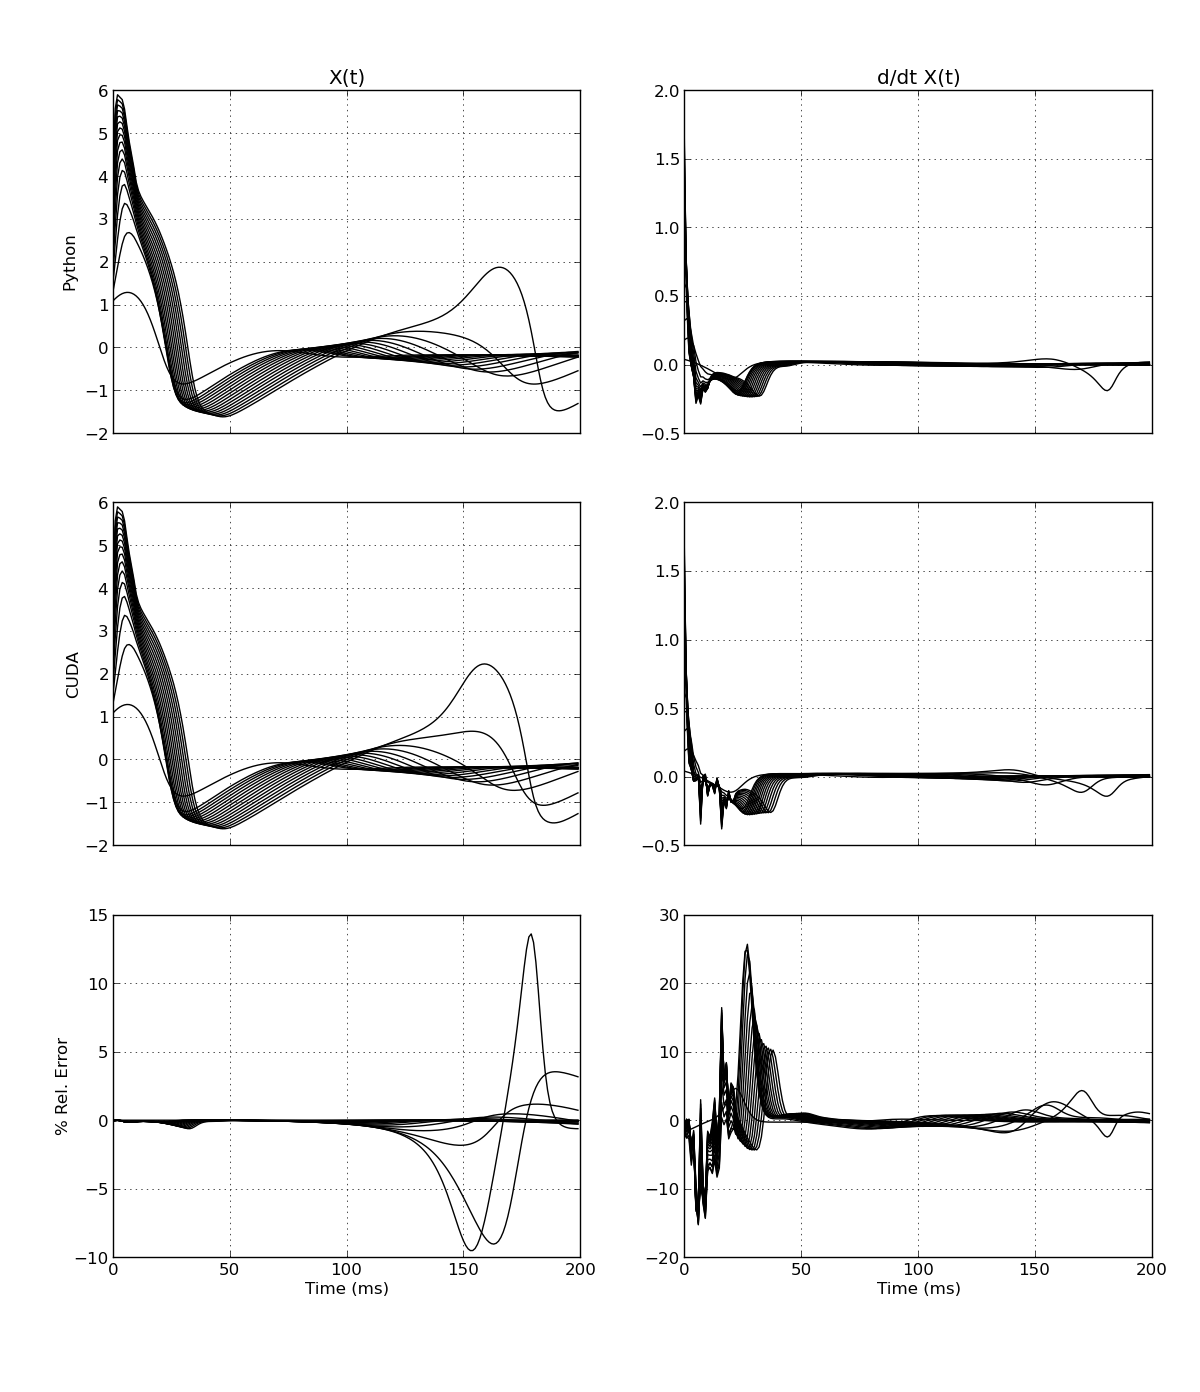
\includegraphics[width=0.48\textwidth]{images/gpu_dxdt.png}}
	\caption{
	Right A typical parameter space exploration, 32 x 32 grid of
	coupling strength (y-axis) v. neural excitability (x-axis).
	This grid of simulations was run on both TVB's Python/NumPy
	implementation and the new GPU backend for 200 ms simulation
	time with otherwise default parameters. The former took ~2
	hours and the latter ~ 1 min. Left Quantitative comparison of
	solutions and instantaneous derivatives is shown for an even
	sampling of the parameter space across k where a = -2, because
	this slice showed the most error on the GPU. 	
	}
	\label{fig:gpu_dxdt}
\end{figure}

 \begin{figure}
	{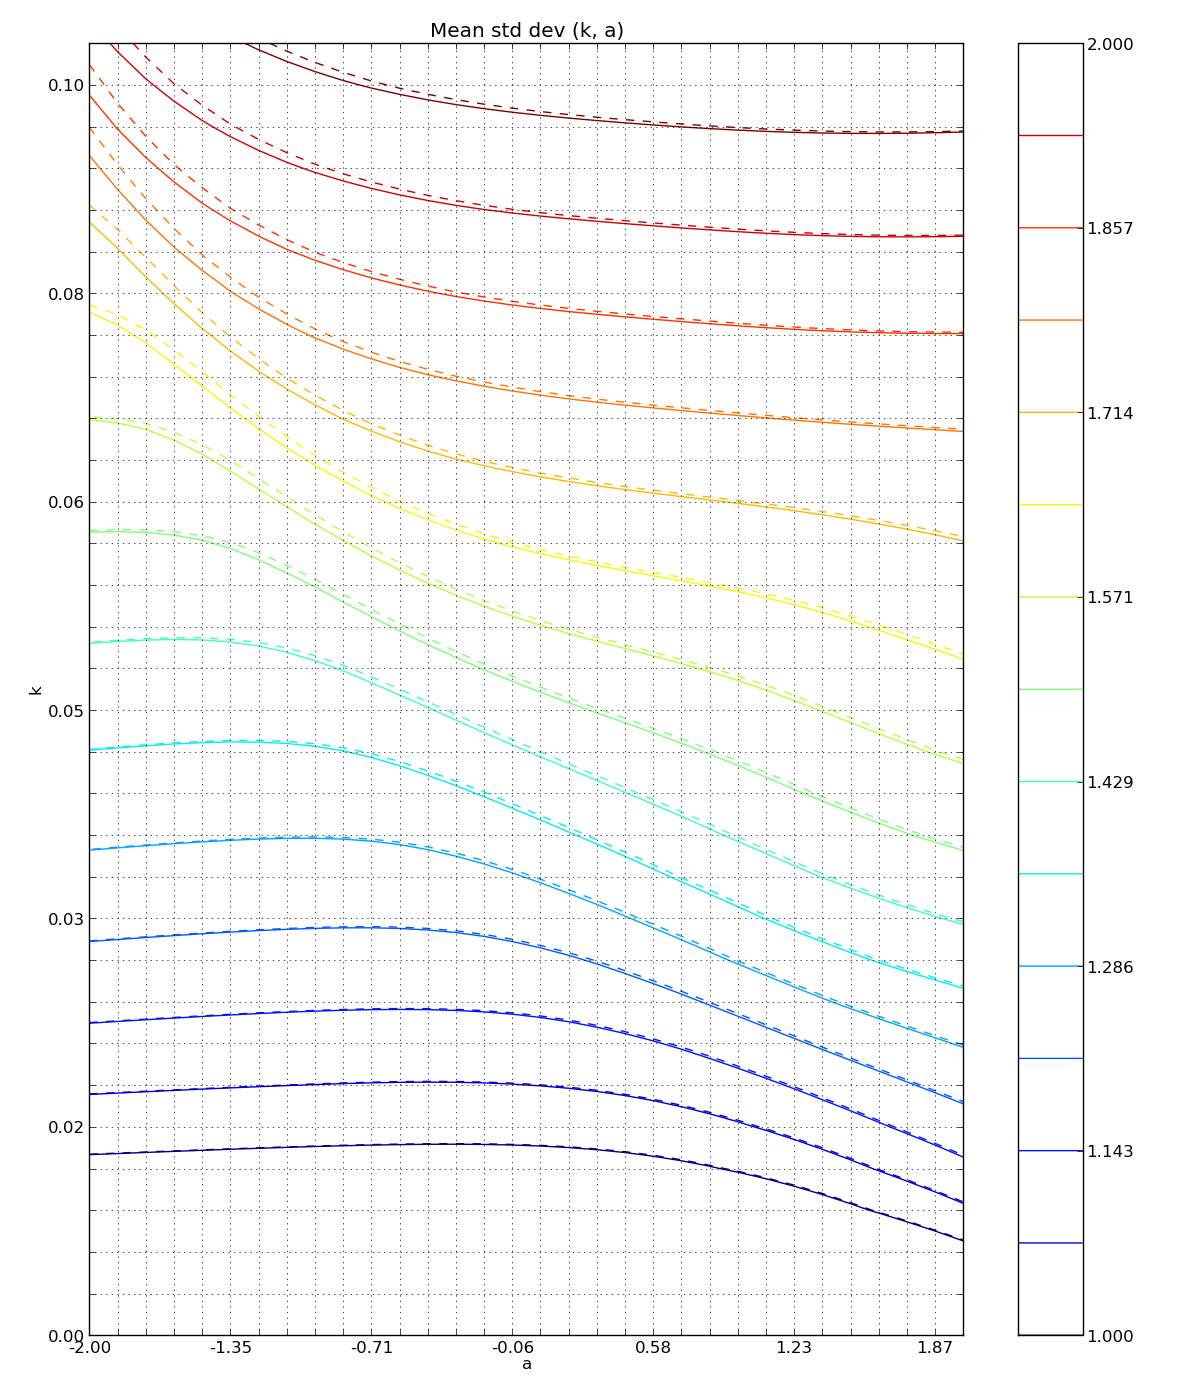
\includegraphics[width=0.48\textwidth]{images/gpu_pse.png}}
	\caption{}
	\label{fig:gpu_pse}
\end{figure}

\note[sk]{One figure or two, re captions}

\note[sk]{Specify hardware (GPU/CPU) and whether Numpy is mkl-linked, to 
    provide a more solid foundation for timing comparisons...}

\note[sk]{It would be interesting to see a longer run (say a few seconds)
    to show if/how-quickly the error grows...}

As can be seen in the listing \note[sk]{can listings be numbered and
labelled...}\note[lp]{Done see example and edit}, the calculations
in native code are performed with 32-bit floating point numbers, and it
is reasonable to ask if this is numerically accurate. In Fig 
\ref{fig:gpu_pse}, we present a parameter space exploration performed with
both the pure Python NumPy simulator and the GPU simulator, showing the 
isocontours of average standard deviation in the parameter space. Some
deviation can be identified visually in parts of the parameter space, and
in in Fig \ref{fig:gpu_dxdt}, we show in more detail time series of 
the Python and GPU solutions.

 \begin{figure}
	{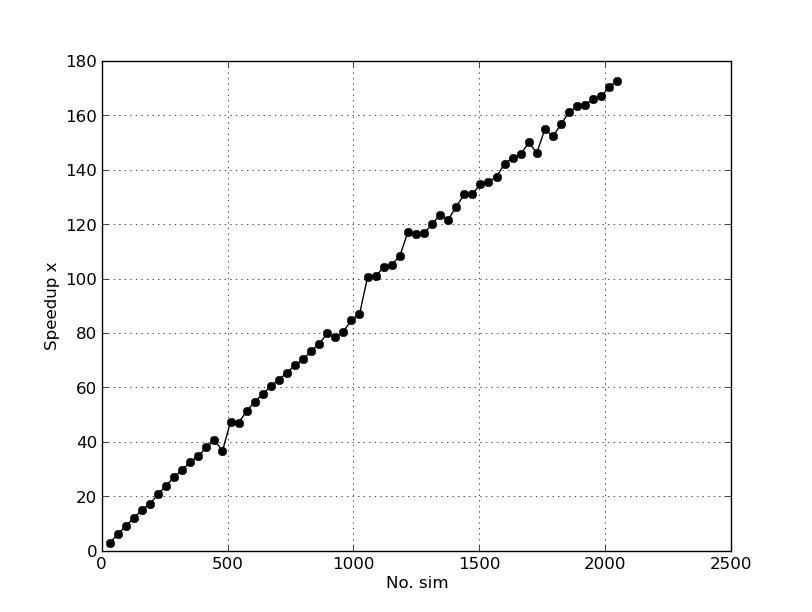
\includegraphics[width=0.48\textwidth]{images/gpu_acceleration.png}}
	\caption{}
	\label{fig:gpu_acceleration}
\end{figure}

This approach allows significant acceleration of parameter sweeps in the
case of the GPU by taking
advantage of the fact that in many cases, only numerical values vary
between different threads and not memory access patterns. Where one of the
dimensions of a parameter sweep implies changing memory access patterns, 
for example conduction speed, it is advantageous to reorder the parameters,
so that such memory varying parameters only change between grids of GPU
threads and not within.

In Fig \ref{fig:gpu_acceleration}, we plot the speedup brought by the GPU
over the Python NumPy simulator as a function of the number of simulations 
performed simulataneously on the GPU.


